We evaluate the proposed approach using a set of four experiments.
A toy problem is first used to study the transfer of learning between two related processes through the shared inducing points.
We then compare the model with existing multioutput models on the tasks of predicting foreign exchange rates and air temperature.
In the final experiment, we test the model on the prediction of robot arms dynamic on a large-scale dataset. 
All experiments are executed on an Intel(R) Core(TM) i7-2600 3.40GHz CPU with 8GB of RAM using Matlab R2012a.
%except for large scale?

\subsection{TOY PROBLEM}
In this toy problem, two related outputs are simulated from the same latent function $sin(x)$ corrupted by independent noises: $y_1(x) = sin(x) + \epsilon$ and $y_2(x) = -sin(x) + \epsilon$, $\epsilon \sim \Normal(0,0.01)$.
The first output has missing observations in the $(-7,-3)$ interval and the second output in the $(4,8)$ interval.
The predictive distributions by our model ($Q = 1$) and independent stochastic GPs (one for each output) are shown in \ref{fig:toy}.
It can be seen that our multioutput model gives perfect prediction in the unobserved regions where the independent models fail to interpolate despite having the same set of inducing inputs.
This confirms that transfer of information from one output to another via collaborative learning of the posterior over the shared inducing inputs.
Furthermore, the inference procedure learned that the weights are $w_{11} = 1.07$ and $w_{21} = -1.06$ which precisely reflects the correlation between the two outputs.

\begin{figure*}
\centering
\begin{tabular}{cccc}
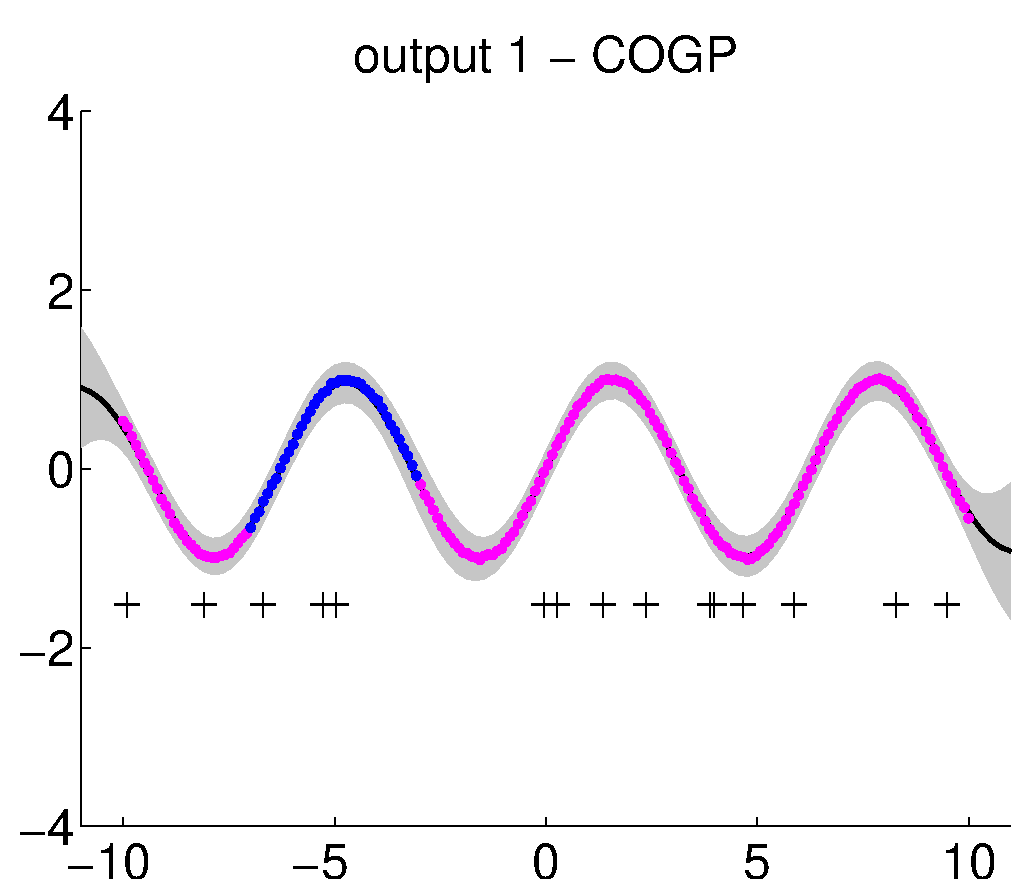
\includegraphics[scale=0.2]{figures/toy-slfm-y1.eps} &
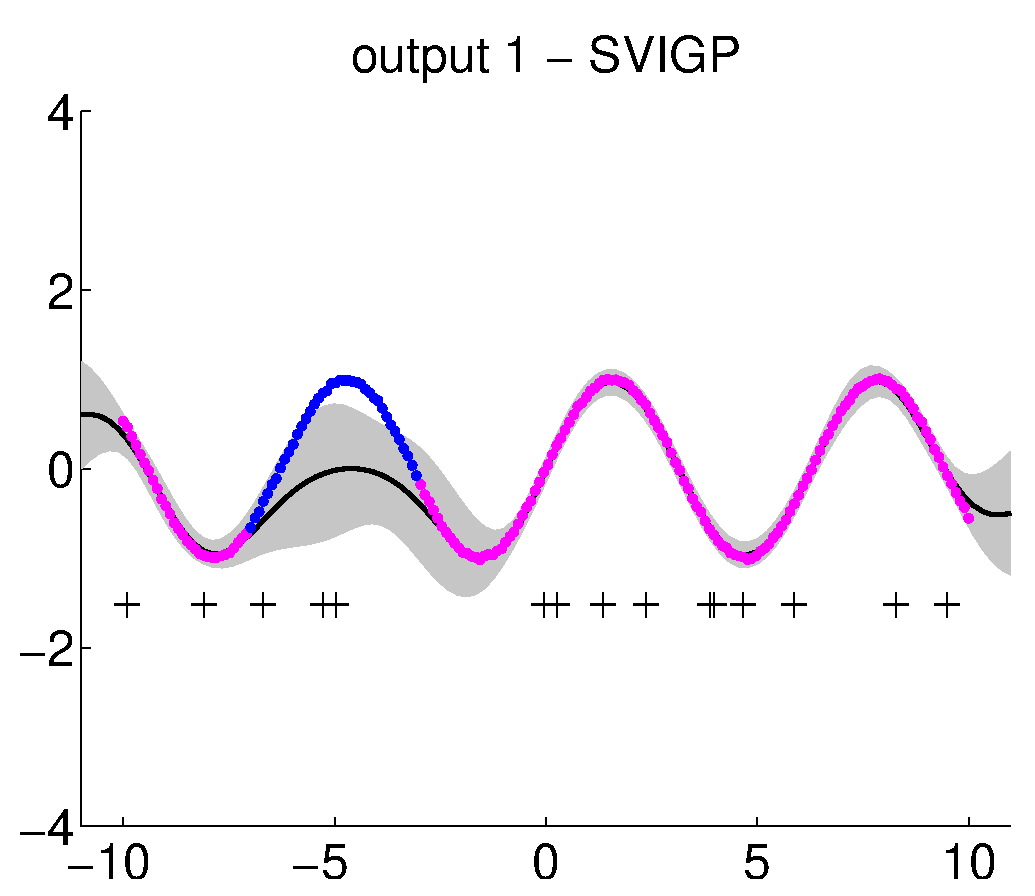
\includegraphics[scale=0.2]{figures/toy-svigp-y1.eps} &
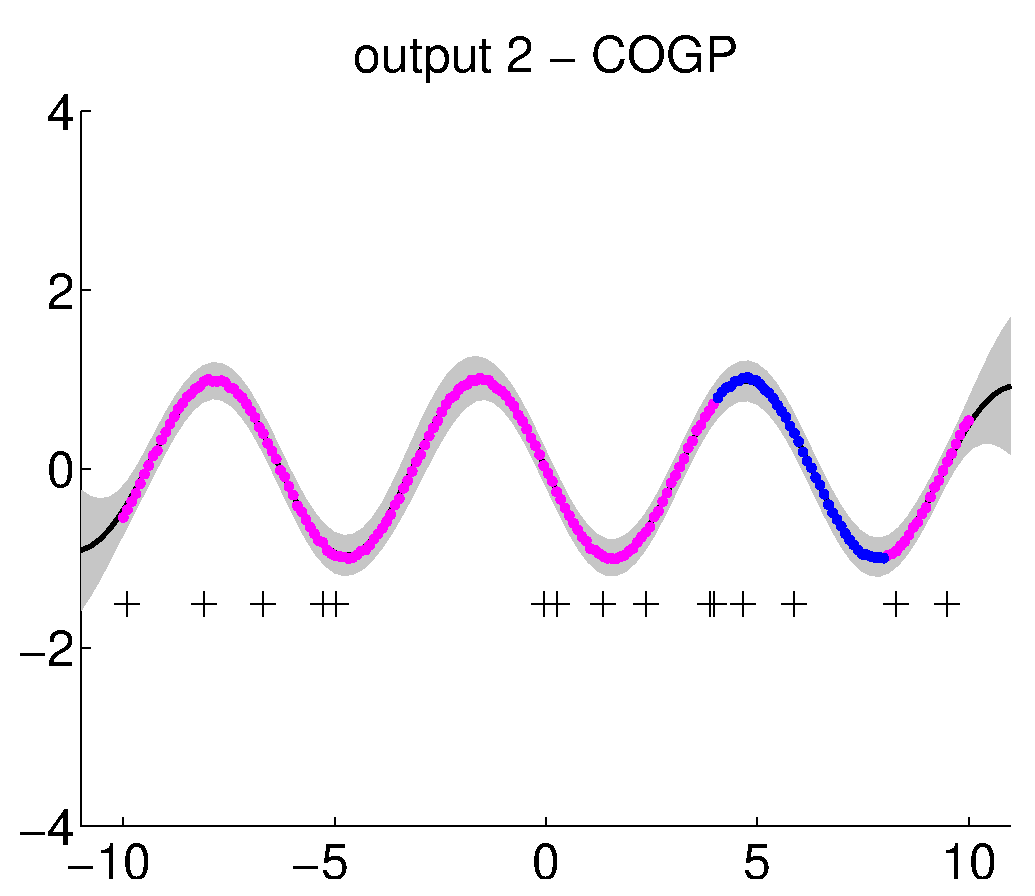
\includegraphics[scale=0.2]{figures/toy-slfm-y2.eps} &
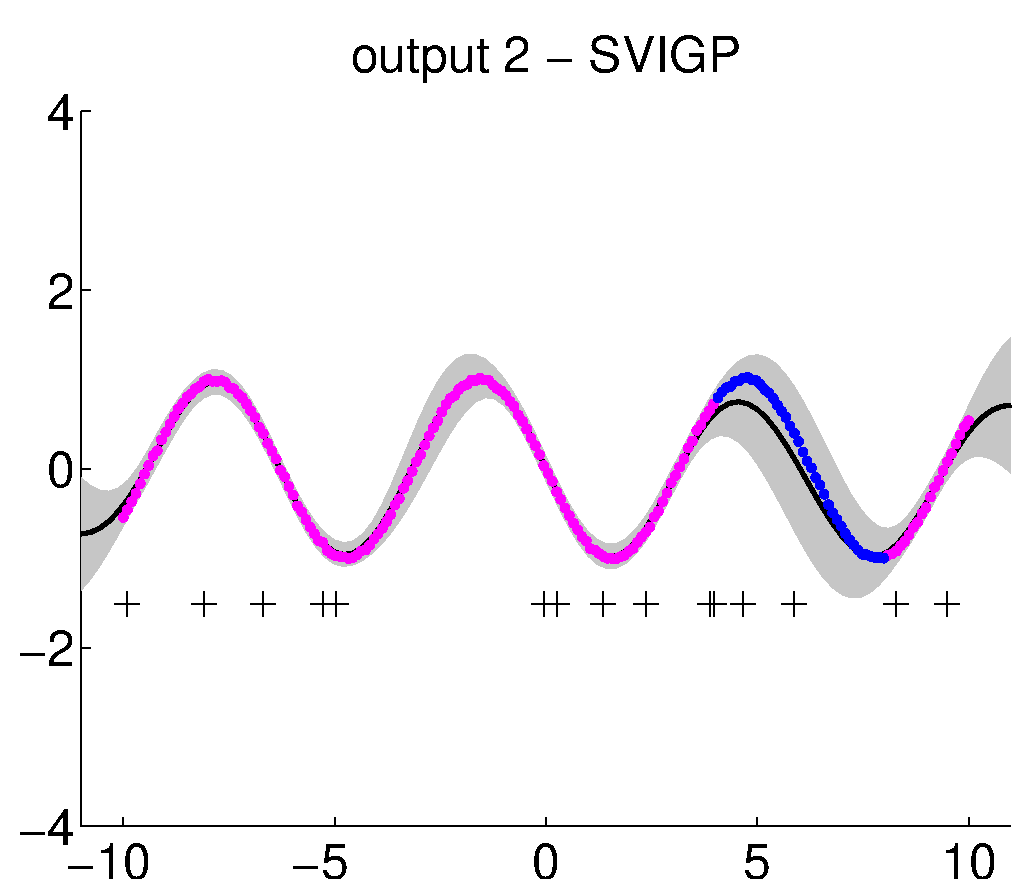
\includegraphics[scale=0.2]{figures/toy-svigp-y2.eps}
\label{fig:toy}
\end{tabular}
\caption{Predictive distributions of the multioutput GPs (first and third figure) and independent GPs using stochastic variational inference (second and last figure) for the  toy problem. Solid black line: predictive mean; grey bar: two standard deviations; magenta dots: real observations; blue dots: missing data. The black crosses show the locations of the inducing inputs.}
\label{fig:toy}
\end{figure*}

\subsection{FOREIGN EXCHANGE RATE PREDICTION}
The application considered here is to predict the foreign exchange rate w.r.t the US dollar of the top 10 international currencies (CAD, EUR, JPY, GBP, CHF, AUD, HKD, NZD, KRW, and MXN) and 3 precious metals (gold, silver, and platinum)\footnote{Data is available at http://fx.sauder.ubc.ca/data.html}. 
The setting of our experiment described here is identical to that in \citet{alvarez2010efficient}.
The dataset contains all the data available for the 251 working days in the year of 2007.
There are 9, 8, and 42 days of missing values  for gold, silver, and platinum, respectively.
We remove from the data the exchange rate of CAD on days 50-100, JPY on day 100-150, and AUD on day 150-200.
Note that these 3 currencies are from very different geographical locations. 
The 153 points extracted is used for testing and the remaining 3051 data points is used for training.
Since the missing data is long contiguous sections, the objective is to evaluate the capacity of the model to impute the missing currency values based on other currencies.
%todo: batch size, learn rate (maybe at the beginning of experiments)

For preprocessing we normalized the outputs to have zero mean and unit variance.
Since the exchange rates are driven by a small number of latent market forces \citet{alvarez2010efficient}, we tried different values of $Q = {1,2,3}$ and selected $Q = 2$ which gave the best model evidence (ELBO).
We used the squared-exponential covariance function for the shared processes and a noise covariance function for the independent process of each output.
The inducing inputs $(M = 100)$ are randomly selected from the training set and fixed throughout training.

The predictive distributions by our model (Figure \ref{fig:fx}) exhibit similar behavior to those by the convolved model with inducing kernels in \citet{alvarez2010efficient}.
In particular, both models perform better at capturing the strong depreciation of the AUD than the fluctuations of the CAD and JPY currency.
Our investigation of the dataset found that 4 other currencies (GBP, NZD, KRW, MXN) also experienced the same trend during the days 150 - 200.
This was effectively used by the model to extrapolate the values of the AUD.

%todo: result for independent gps
We also report in Table \ref{tab:fx} the predictive accuracy of our model compared to the convolved GPs model with exact inference \citet{alvarez-lawrence-nips-08} (CGP) and with approximation via the variational inducing kernels \citet{alvarez2010efficient}) (CGPVAR) in addition to using independent GPs (IGP, one for each output).
Our model outperforms both of the CGP variants in terms of standardized mean-squared error (SMSE).
It has lower test likelihood, as measured by the negative log predictive density (NLPD), which is mainly due to the less conservative predictive variance of the exact CGP for the CAD currency.
%The results are averaged across the 3 outputs over 5 repetitions.
% no std because there are 3 outputs but variance is small
Note that the SMSE of CGPVAR is taken from \citet{alvarez2010efficient} while the NLPD was not provided.
Training took only 10 minutes for our model compared to 1.4 hours of the full CGP model.

\setlength{\tabcolsep}{4pt}
\begin{table}[t]
\caption{Performance comparison on the foreign exchange rate dataset. Results are averaged of the 3 outputs over 5 repetitions.}
\label{tab:fx}
\begin{center}
\begin{tabular}{ccc}
\toprule
\textbf{METHOD} & \textbf{SMSE} & \textbf{NLPD} \\ \hline
COGP  & \textbf{0.2125} & -0.8394 \\
CGP & 0.2427 & \textbf{-2.9474} \\
IGP & 0.5996 & 0.4082 \\
CGPVAR & 0.2795 & NA \\
%ICM & 0.3927 &
\bottomrule
\end{tabular}
\end{center}
\end{table}

\begin{figure*}
\centering
\begin{tabular}{ccc}
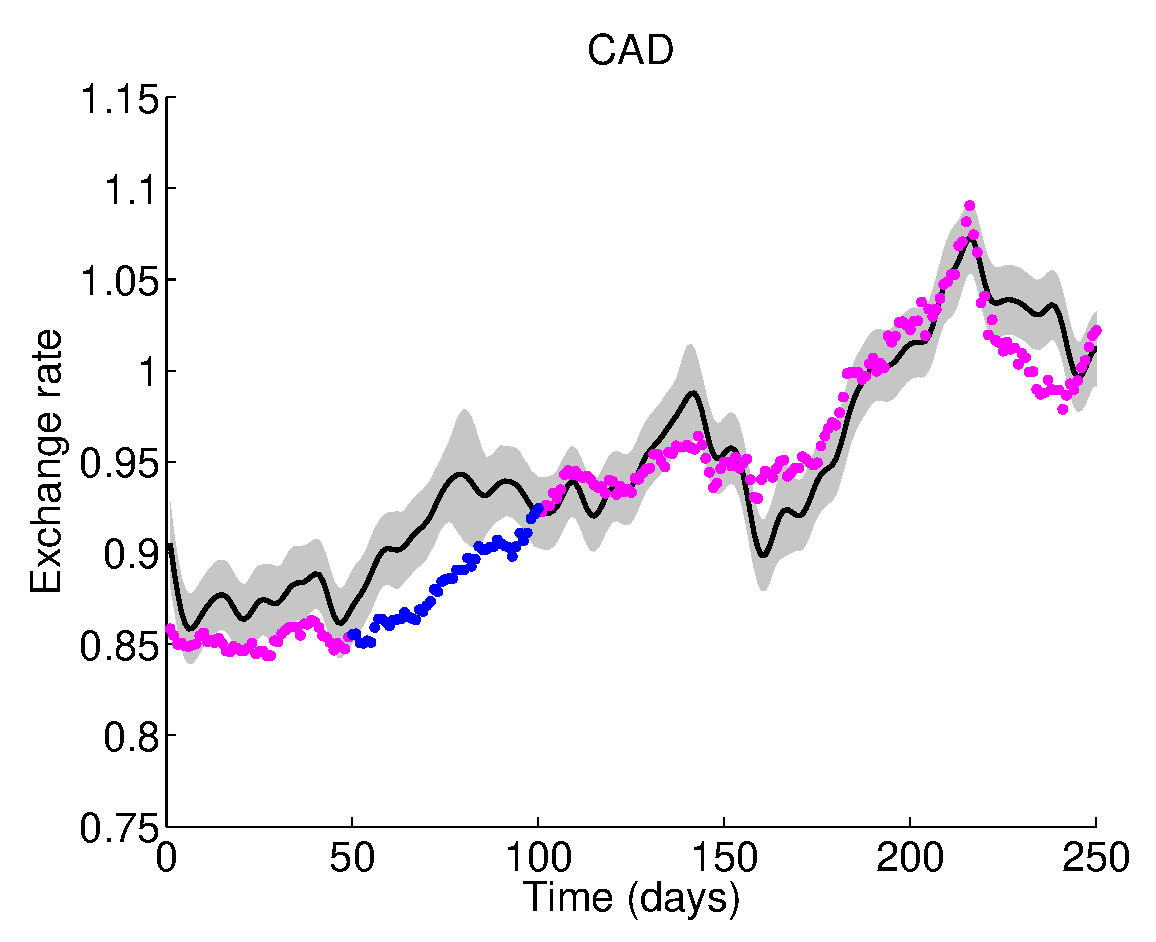
\includegraphics[scale=0.3]{figures/fxCAD.eps} &
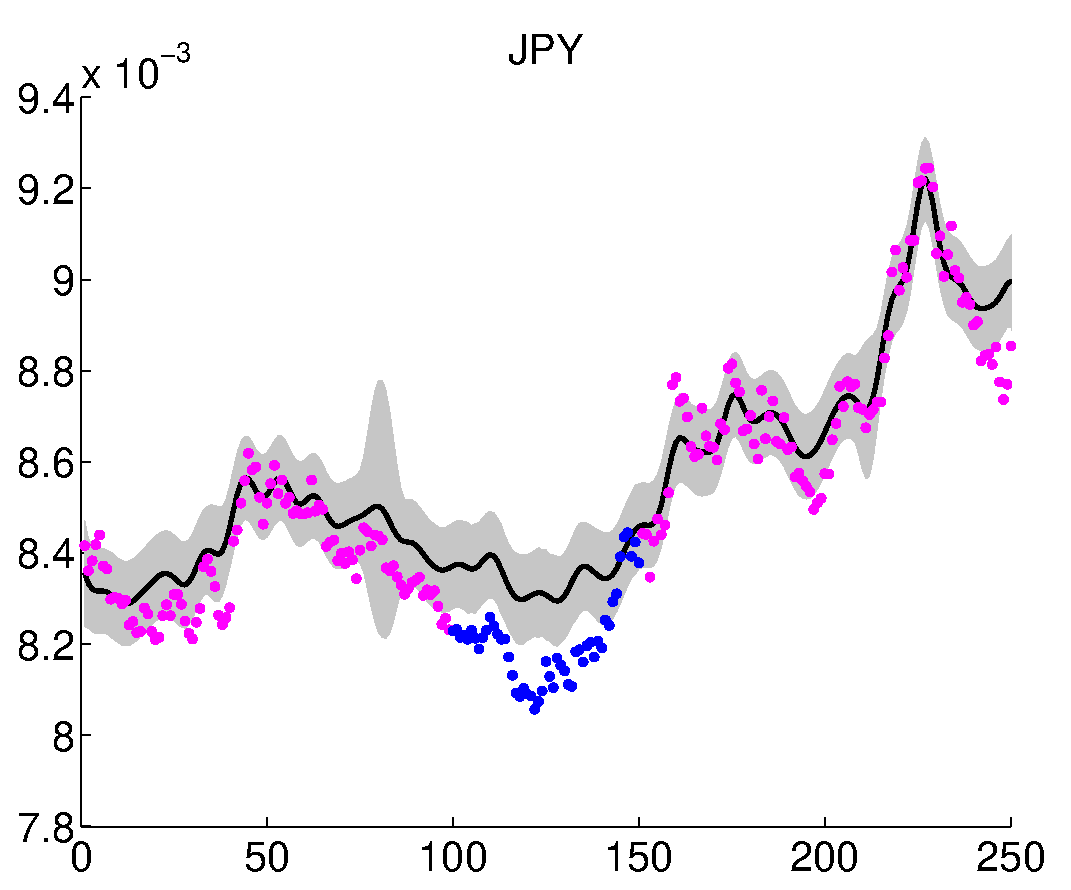
\includegraphics[scale=0.3]{figures/fxJPY.eps} &
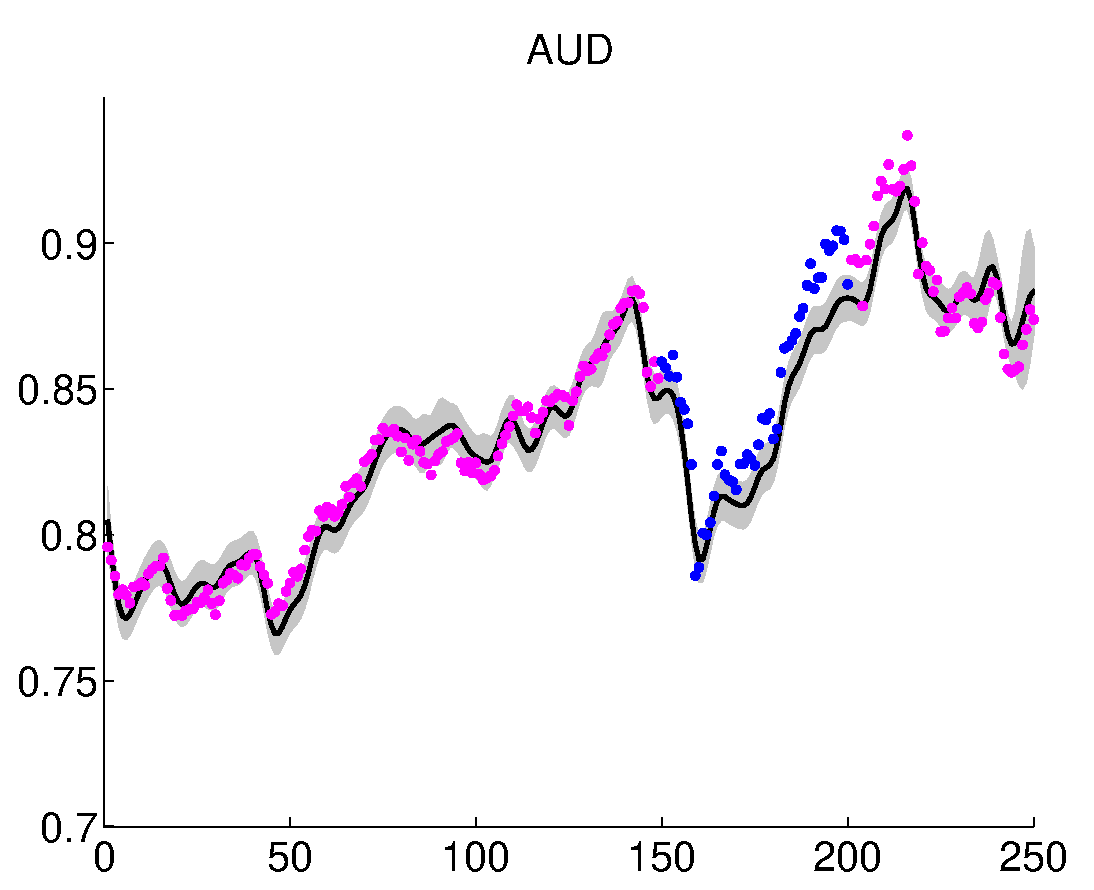
\includegraphics[scale=0.3]{figures/fxAUD.eps}
\end{tabular}
\caption{Real observations and predictive distributions for CAD (left), JPY (middle), and AUD (right). The color coding scheme is the same as in figure \ref{fig:toy}.}
\label{fig:fx}
\end{figure*}

\subsection{AIR TEMPERATURE PREDICTION}
Next, we consider the task of predicting air temperature at 4 different locations in the south coast of England. 
The data is gathered from a network of weather sensors (named Bramblemet, Sotonmet, Cambermet, and Chimet), each of which measures several environmental variables \citet{osborne2008towards}\footnote{Data is available at seperate web pages, see e.g. http://www.bramblemet.co.uk}.
%The sensors are close geographically so we can expect correlation in air temperature.
We selected the sensor signal for air temperature during the period from July 10 to July 15, 2013.
The sensors record measurements every 5 minutes, resulting in a maximum of 4320 observations.
There are missing data for Bramblemet (100 points), Chimet (15 points), and Sotonmet (1002 points), possibly due to network outages or hardware failures.
We further simulated failure of the sensors by removing the observations from the time periods [10.2 - 10.8] for Cambermet and [13.5 - 14.2] for Chimet.
The removed data comprises 375 data points, which is used for testing, and the remaining data consisting of 15,788 points is used for training.
Similar to the previous experiment, the objective is to evaluate the ability of the model to use the signals from the functioning sensors to extrapolate the missing signals.

For pre-processing we normalized the outputs to have zero mean and unit variance.
The inducing inputs $(M = 200)$ are randomly selected from the training set and fixed throughout training.
The number of latent processes is $Q = 2$ for both our model and the CGP model.

The real data and the predictive distributions by 3 models (COGP, CGP with exact inference, and independent GPs) are shown in Figure \ref{fig:weather}.
It is clear that the independent GPs model is clueless in the test regions and thus simply uses the average temperature as its prediction.
For Cambermet, both COGP and CGP can capture the rising in temperature from the morning till the afternoon and the fall afterward.
For Chimet, both models perform poorly but CGP more so as it falsely predicts  wild fluctuations that are non-existent in the data. 
Note that the two latent processes learned by our model indeed correspond to different patterns in the data: one process has the inverse lengthscale of 136 which captures the global increase in temperature during the training period while the other has the inverse lengthscale of 0.5 to model the local variations within a single day.
The comparative performance of the models are summarized in Table \ref{tab:air}, which further supports the qualitative analysis that our model outperforms CGP.
%All results are averaged of the 2 outputs over 5 repetitions.
Training of our model took on average 5 minutes compared to 3 hours of CGP with exact inference.

\setlength{\tabcolsep}{4pt}
\begin{table}[t]
\caption{Performance comparison on the air temperature dataset. Results are averaged of 2 outputs over 5 repetitions. }
\label{tab:air}
\begin{center}
\begin{tabular}{ccc}
\toprule
\textbf{METHOD} & \textbf{SMSE} & \textbf{NLPD} \\
\hline
COGP & \textbf{0.1077} & \textbf{2.1712} \\
CGP & 0.1125 & 2.2219 \\
IGP & 0.8944 & 12.5319 \\
\bottomrule
\end{tabular}
\end{center}
\end{table}

\begin{figure*}
\centering
\begin{tabular}{ccc}
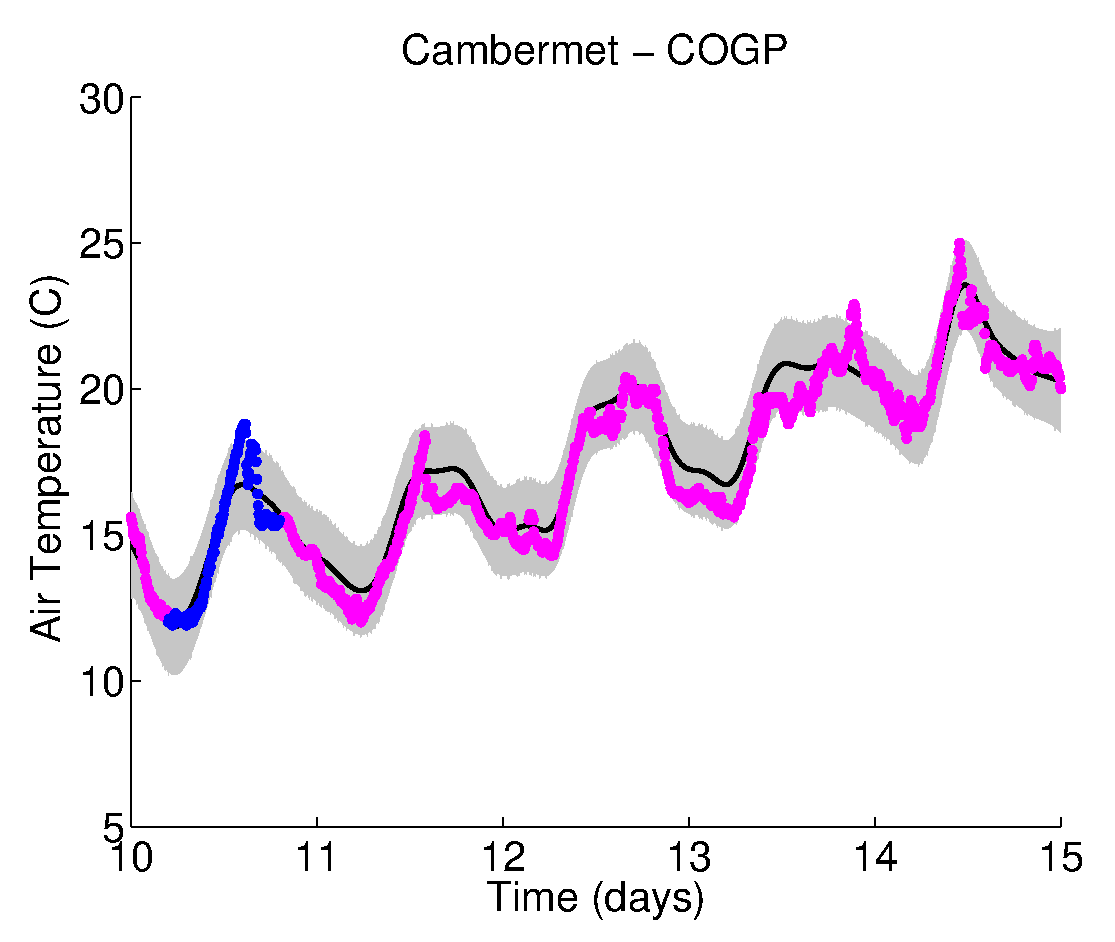
\includegraphics[scale=0.3]{figures/cogp-weatherCambermet.eps} &
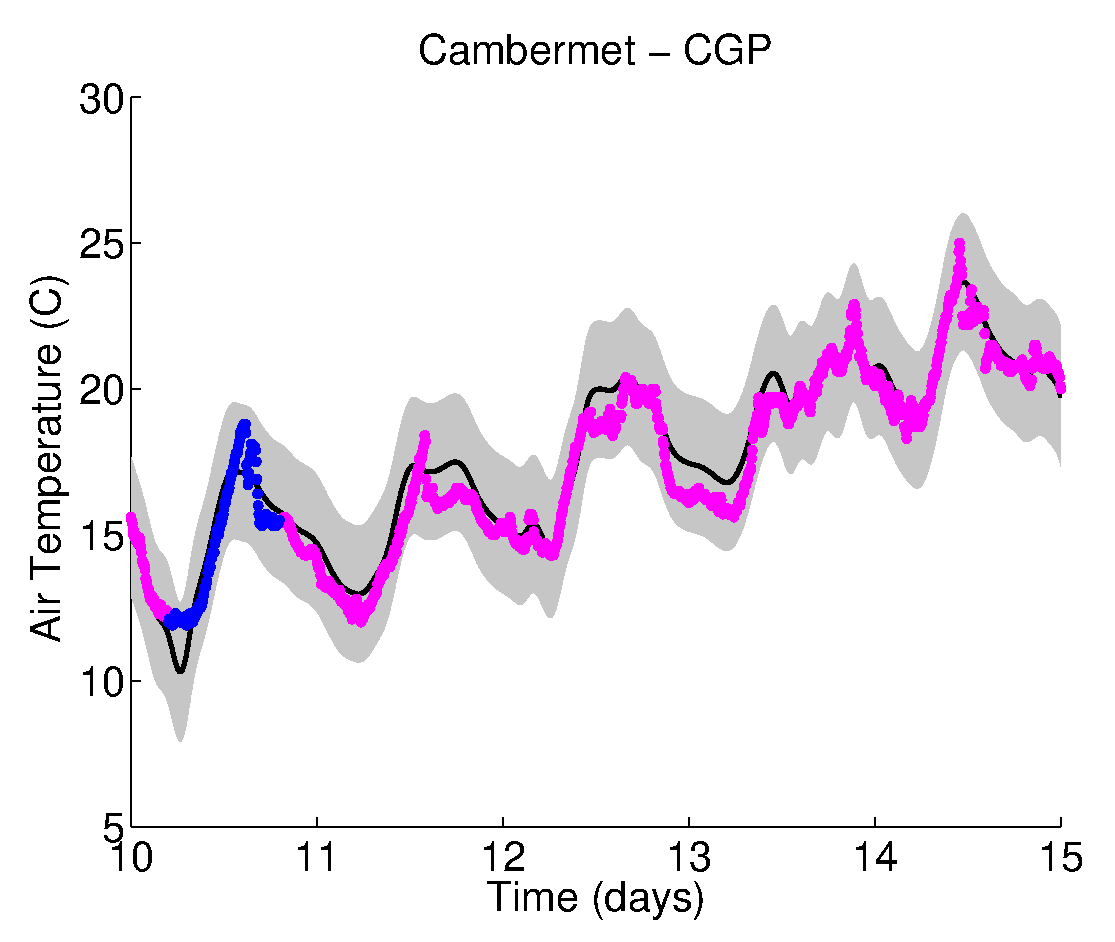
\includegraphics[scale=0.3]{figures/cgp-weatherCambermet.eps} &
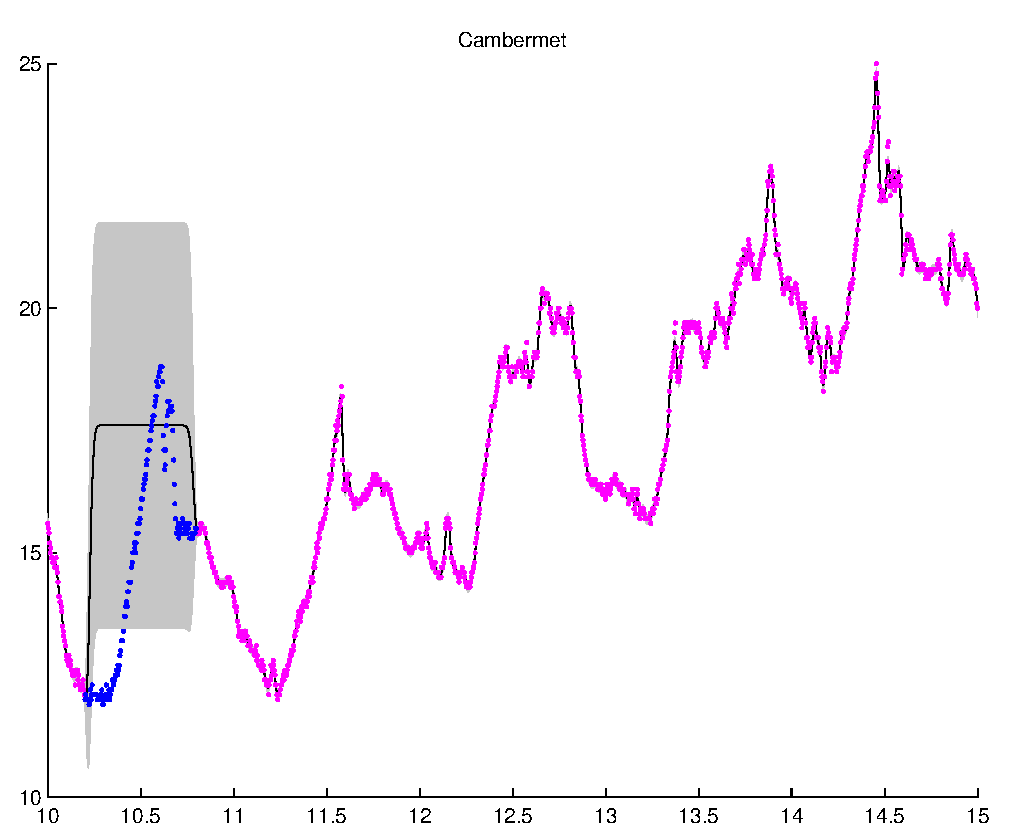
\includegraphics[scale=0.3]{figures/weatherCambermet.eps}
\\
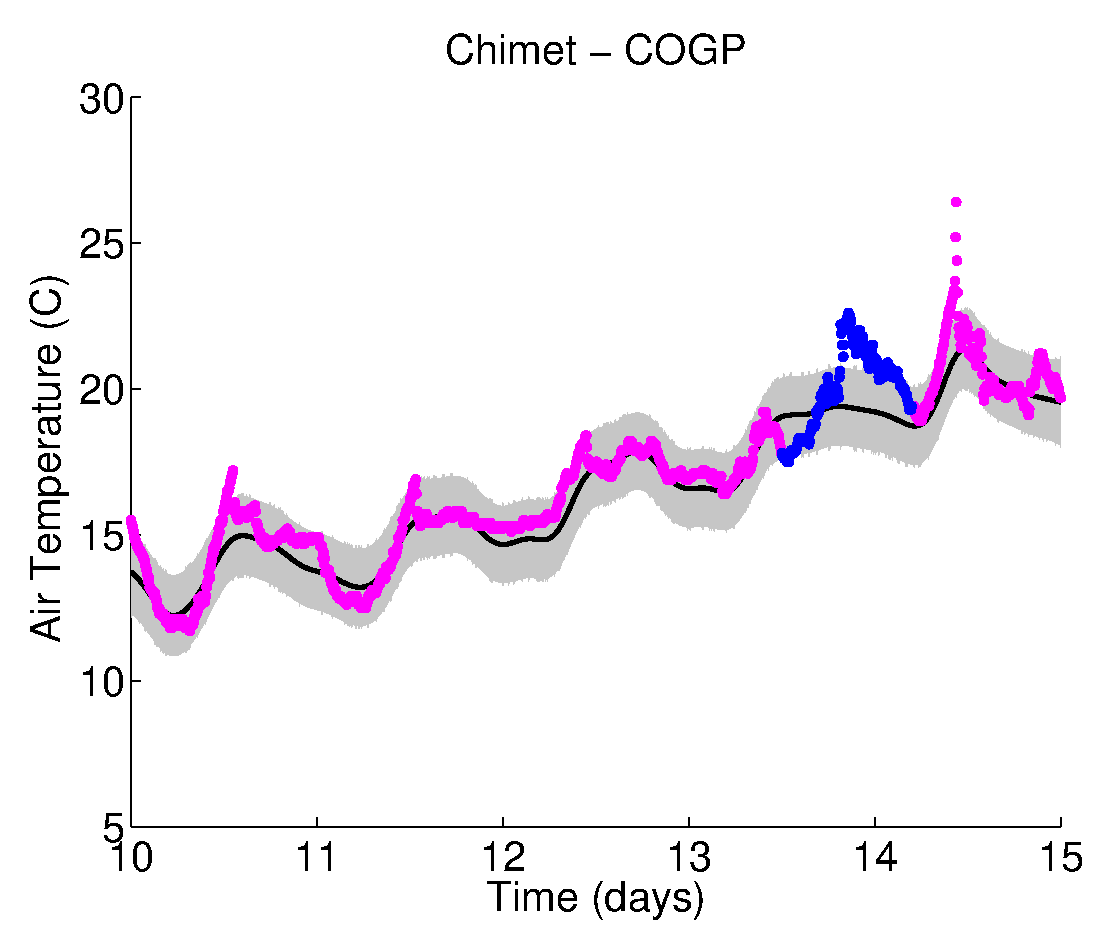
\includegraphics[scale=0.3]{figures/cogp-weatherChimet.eps} &
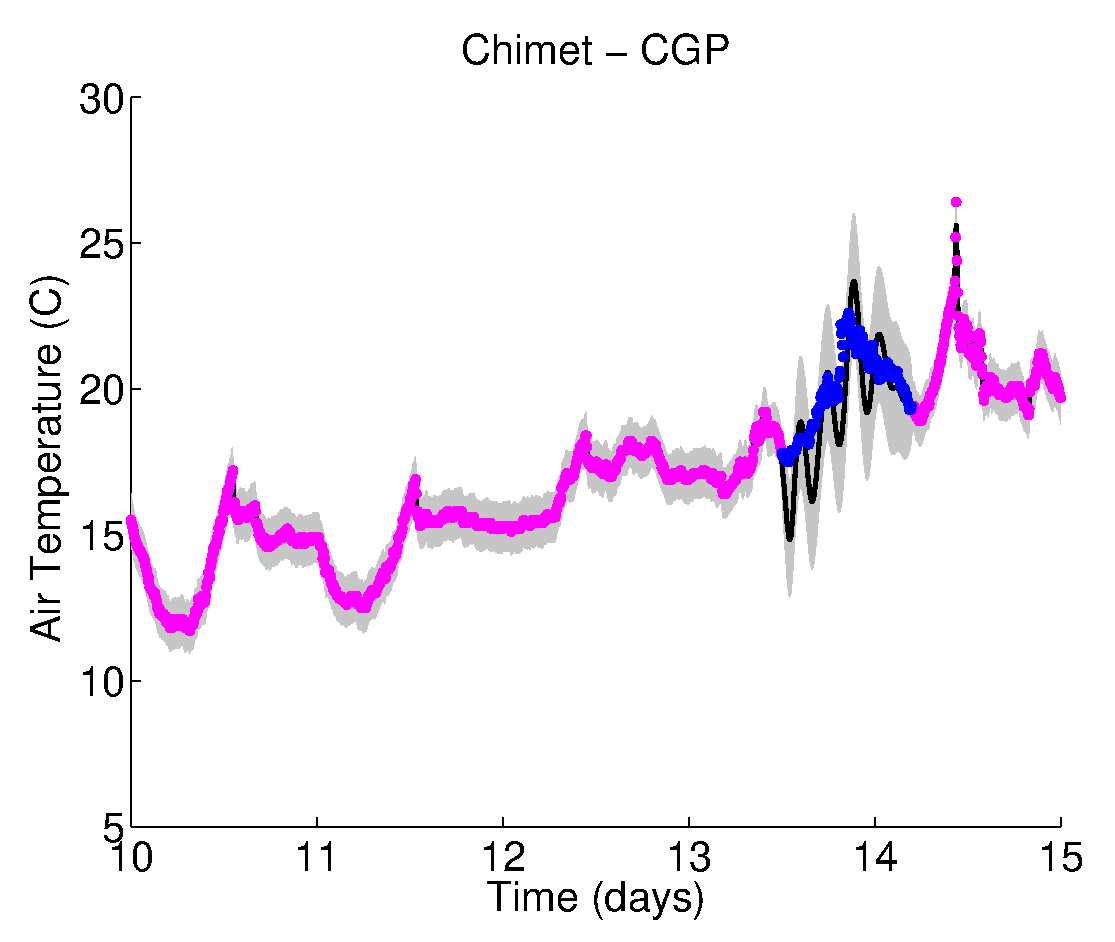
\includegraphics[scale=0.3]{figures/cgp-weatherChimet.eps} &
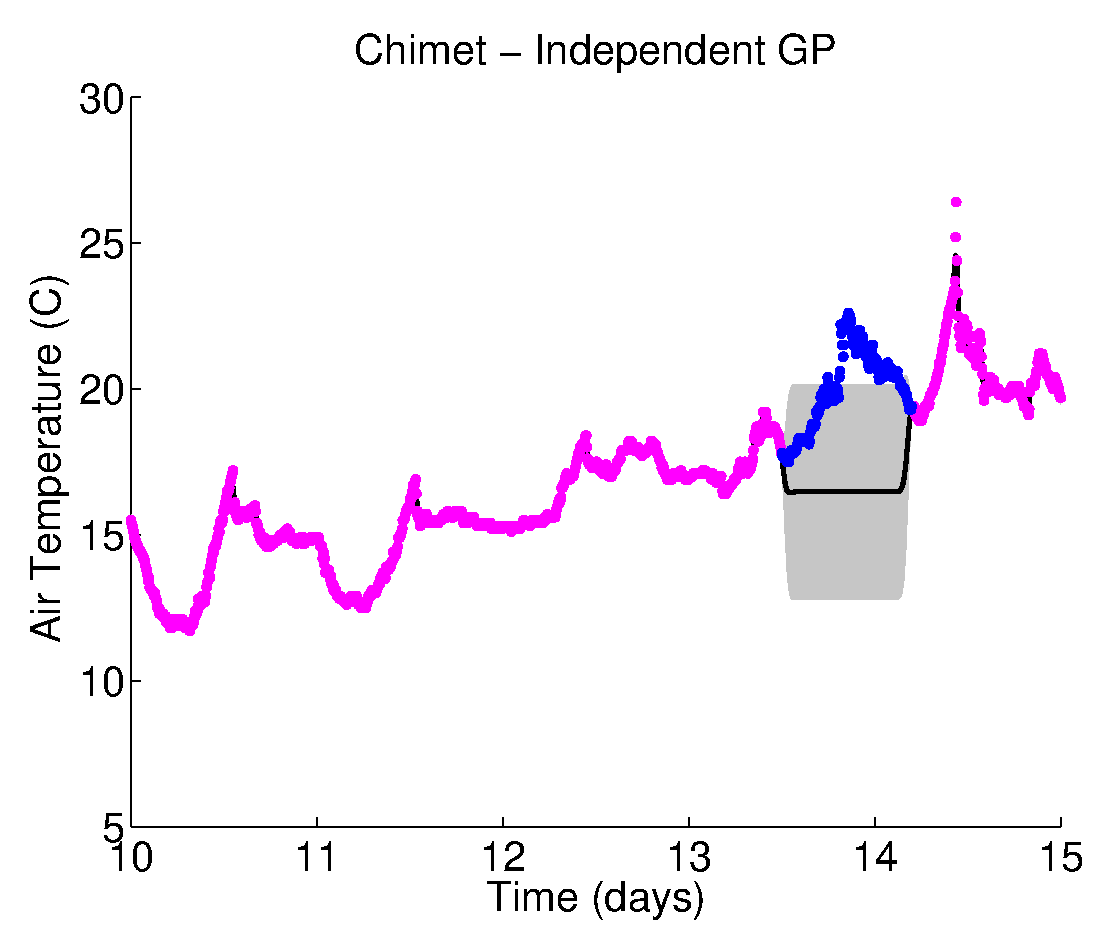
\includegraphics[scale=0.3]{figures/weatherChimet.eps}
\end{tabular}
\caption{Predictive distributions of the multioutput GPs (left column) and full independent GPs (right column) for the air temperature problem.}
\label{fig:weather}
\end{figure*}

\subsection{INVERSE DYNAMICS OF ROBOT ARM}
Our last experiment is with a large scale dataset relating to an inverse dynamics model of a 7-degree-of-freedom anthropomorphic robot arm\footnote{Data is available at http://www.gaussianprocess.org/gpml/data/}.
The data consists of 48,933 mapping from a 21-dimensional input space (7 joints positions, 7 joint velocities, 7 joint accelerations) to the corresponding 7 joint torques.
The problem is strongly nonlinear due to complex superpositions of sine and cosine functions in robot dynamics \citet{vijayakumar2000locally}.
Furthermore, exploratory analysis using standard GP with automatic relevance determination suggests that all of the 21 dimensions are relevant.
We consider here the task of joint learning for the $4$th and $7$th outputs.
Note that previous work (see e.g. \citet{rasmussen-williams-book},  \citet{vijayakumar2000locally}) on this dataset has only dealt with learning  a single output.
We used the same training/testing split as in \citet{rasmussen-williams-book}, resulting in a training set of 88,968 observations and a test set of 8,898 observations.

Since none of the existing multioutput models are applicable to this problem, we compare with two baselines which learn each output independently.
The first is the subset of data approach where a subset of 1000 data points (for each output) is randomly sampled for training. 
We call this method SOD1000.
The second baseline is the sparse GP with stochastic variational inference \citet{hensmangaussian} using 500 inducing inputs, which we refer to as SVIGP.
The outputs are normalized and the squared exponential with ARD covariance function is used for all methods.
In case of COGP, this mean the shared process (we used $Q = 1$) and each of the independent processes have this same covariance function.

The predictive performance of the methods are given in Table \ref{tab:robotarm}.
The results are averaged of the 2 outputs over 5 repetitions.
Both COGP and SVIGP using 500 inducing inputs significantly outperform SOD in terms of the mean absolute error (MAE) but have lower predictive likelihood.

\begin{table}[t]
\caption{Performance comparison on the robot arm dataset. In the two bottom lines, standard GP is applied to output 1 and the remaining method is applied to output 2. Results are averaged over 5 repetitions.}
\label{tab:robotarm}
\begin{center}
\begin{tabular}{lcccc}
\toprule
& \multicolumn{2}{c}{\textbf{OUTPUT 1}} & \multicolumn{2}{c}{\textbf{OUTPUT 2}} \\ \cmidrule(r){2-5}
\textbf{METHOD} & \textbf{SMSE} & \textbf{NLPD} & \textbf{SMSE} & \textbf{NLPD}\\ 
 \midrule
COGP, learn z & \textbf{0.2631} & \textbf{3.0600} & 0.0127 & \textbf{0.8302} \\
COGP, fix z & 0.2821& 3.2281 & 0.0131 & 0.8685 \\
GP, SVIGP & 0.3119 & 3.2198 & \textbf{0.0101} & 1.1914 \\
GP, SOD & 0.3119 & 3.2198 & 0.0104 & 1.9407 \\
\bottomrule
\end{tabular}
\end{center}
\end{table}

\subsubsection{Impact of Optimizing the Inducing Inputs}
% table for smses, nlpds, training tiem
\begin{figure}
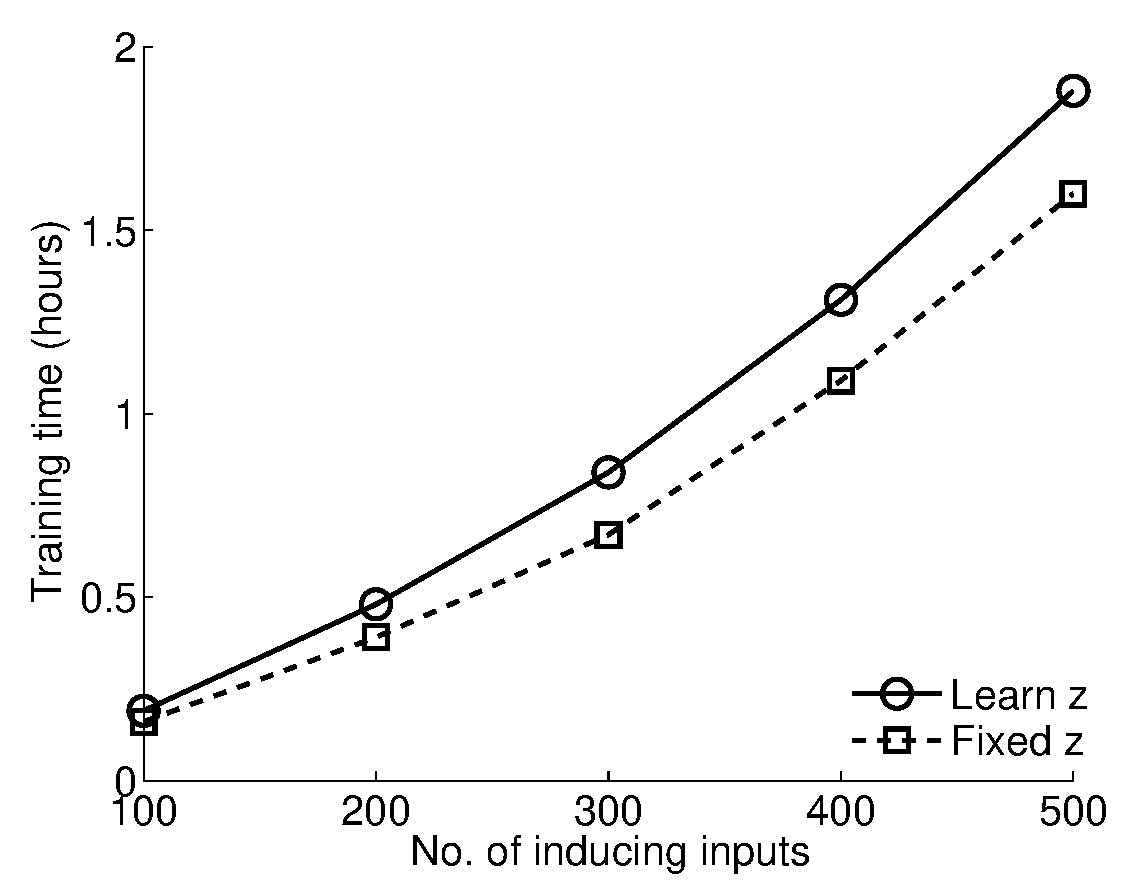
\includegraphics[scale=0.4]{figures/sarcosTime.eps}
\caption{The cost of optimizing versus fixing the inducing inputs.}
\label{fig:time}
\end{figure}
